\section{Aprendix}
\subsection{Pre-Epidemic graphs}
\begin{figure}[H]
\caption{Policy Functions Educated Buyers}
\hspace{-2.0cm}
\begin{center}
\begin{tabular}{cc}
\multicolumn{1}{c}{(a) Value function} &  
\multicolumn{1}{c}{(b) Assets function} \\
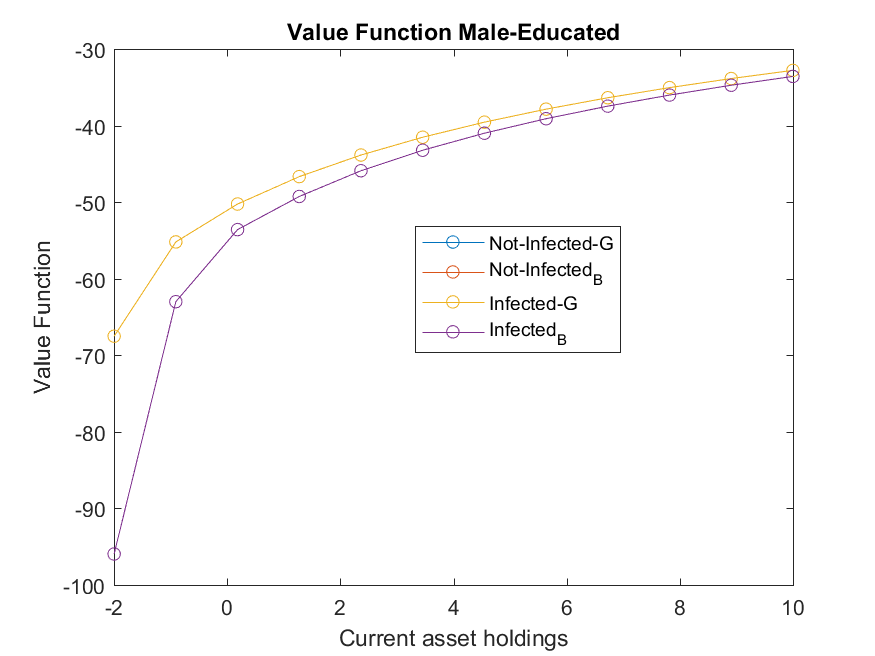
\includegraphics[angle=0,width=.5\textwidth]{figures/FIG1.png}   & 
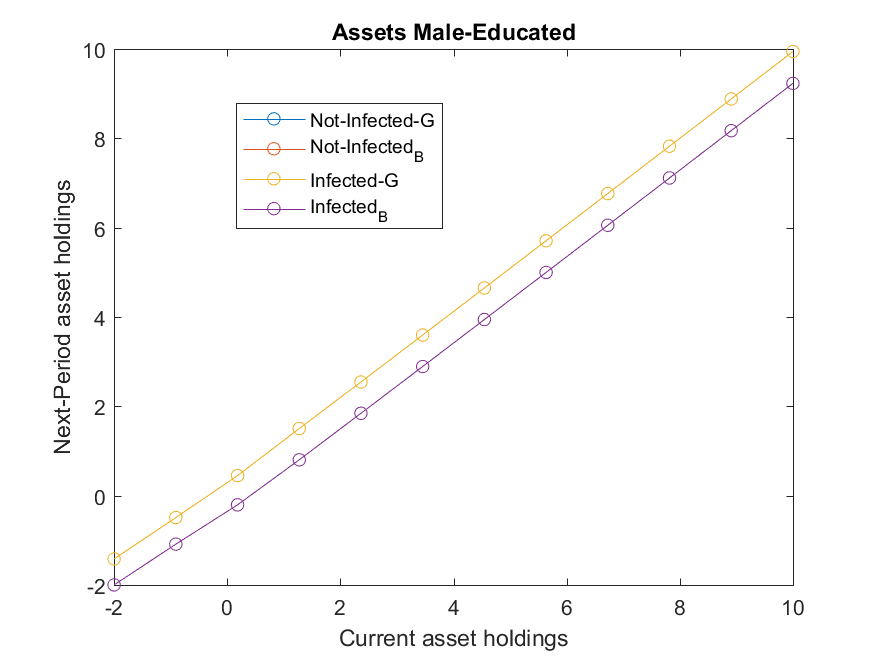
\includegraphics[angle=0,width=.5\textwidth]{figures/FIG3.png} \\
\multicolumn{1}{c}{(c) Consumption function} &  
\multicolumn{1}{c}{(d) Sex consumption function } \\
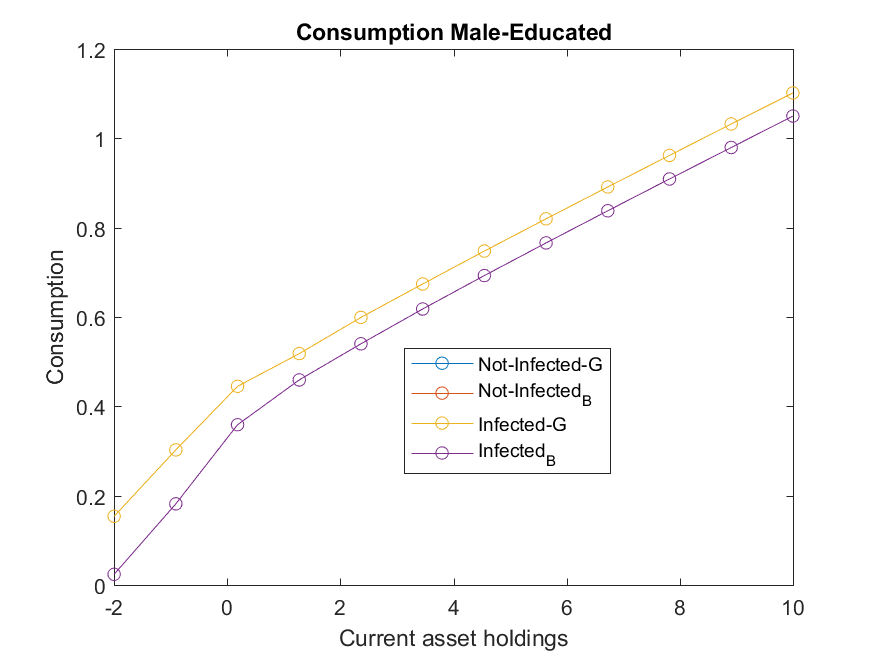
\includegraphics[angle=0,width=.5\textwidth]{figures/FIG2.png}   & 
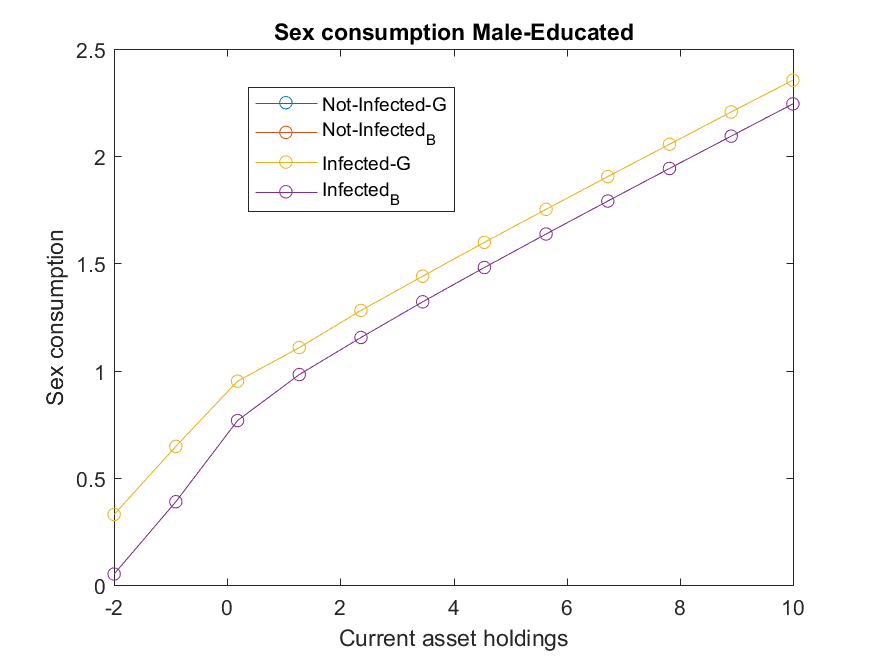
\includegraphics[angle=0,width=.5\textwidth]{figures/FIG4.png} \\
%\multicolumn{1}{c}{(a) Value function} &  
%\multicolumn{1}{c}{(b) Assets function} \\
\end{tabular}
\end{center}
\label{fig:2}
\end{figure}

\begin{figure}[H]
\caption{Policy Functions Educated Sellers}
\hspace{-2.0cm}
\begin{center}
\begin{tabular}{cc}
\multicolumn{1}{c}{(a) Value function} &  
\multicolumn{1}{c}{(b) Asset function} \\
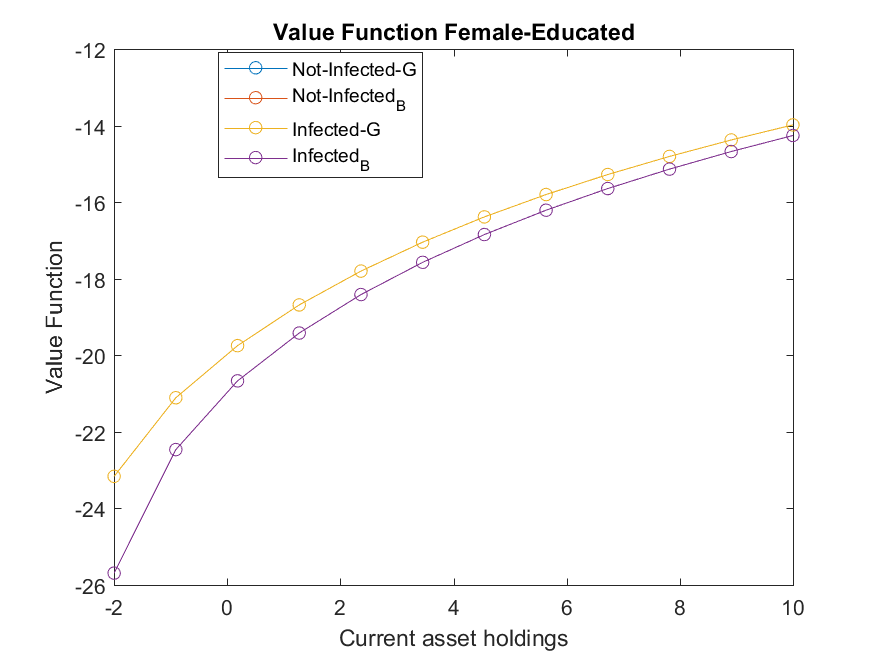
\includegraphics[angle=0,width=.5\textwidth]{figures/FIG5.png}   & 
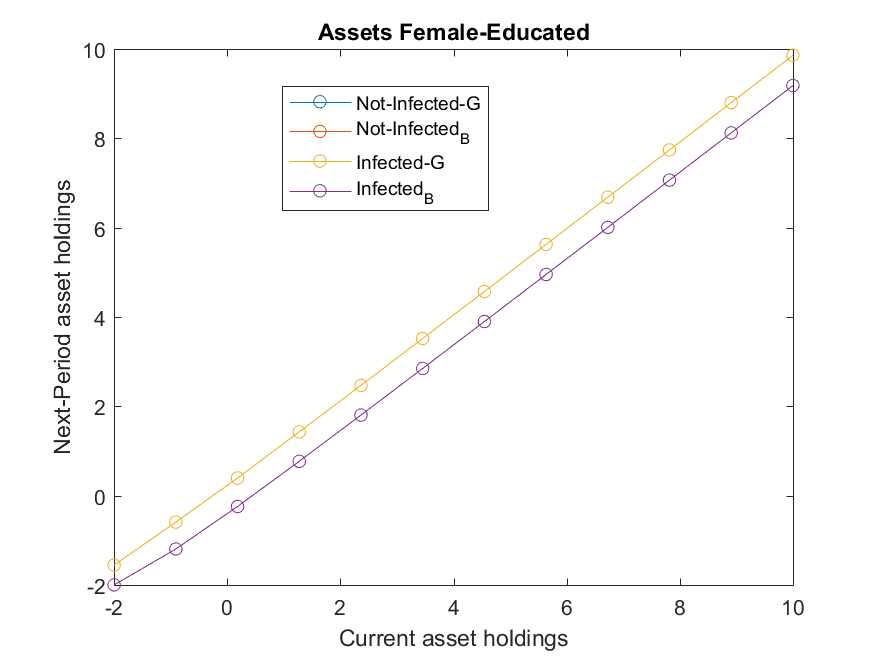
\includegraphics[angle=0,width=.5\textwidth]{figures/FIG7.png} \\
\multicolumn{1}{c}{(c) Consumption function} &  
\multicolumn{1}{c}{(d) Sex Production function } \\
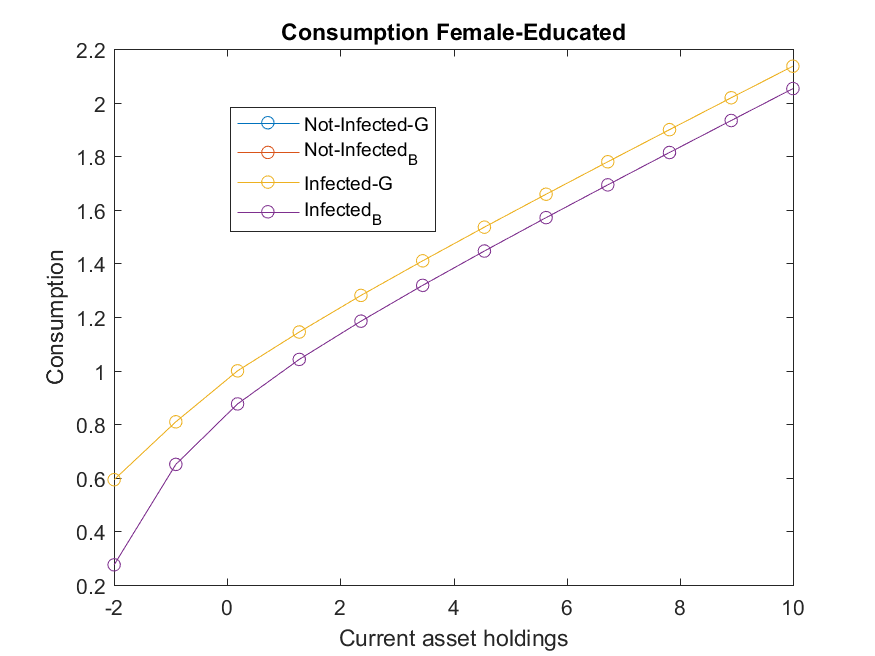
\includegraphics[angle=0,width=.5\textwidth]{figures/FIG6.png}   & 
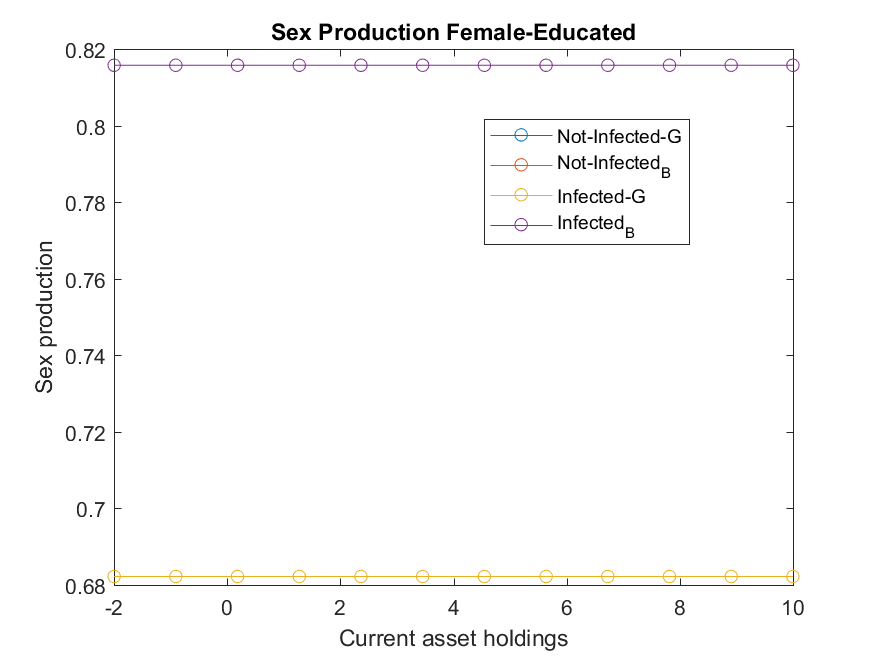
\includegraphics[angle=0,width=.5\textwidth]{figures/FIG8.png} \\
\end{tabular}
\end{center}
\label{fig:3}
\end{figure}



\begin{figure}[H]
\caption{Comparison plots}
\hspace{-2.0cm}
\begin{center}
\begin{tabular}{cc}
\multicolumn{1}{c}{(a) Asset Policy Functions} &  
\multicolumn{1}{c}{(b) Consumption Policy Functions} \\
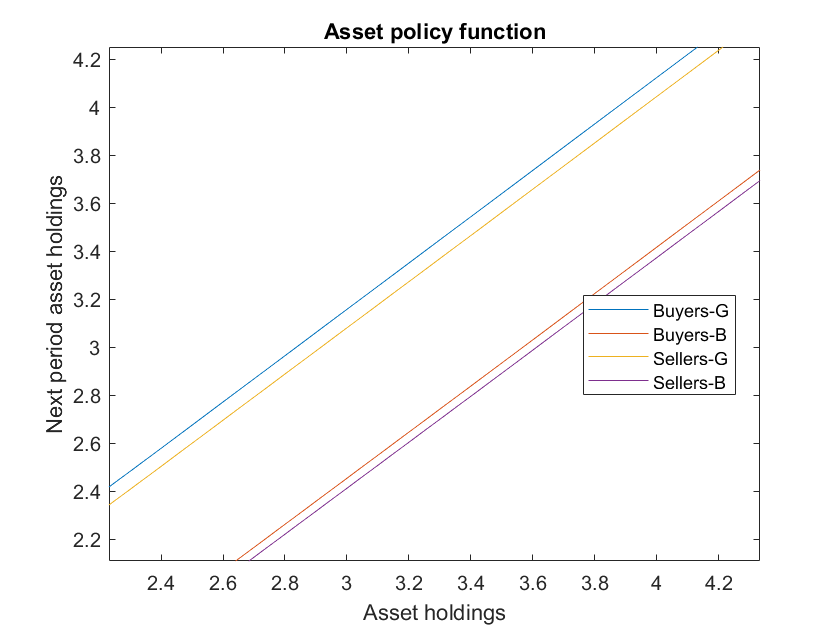
\includegraphics[angle=0,width=.5\textwidth]{figures/FIG11.png}   & 
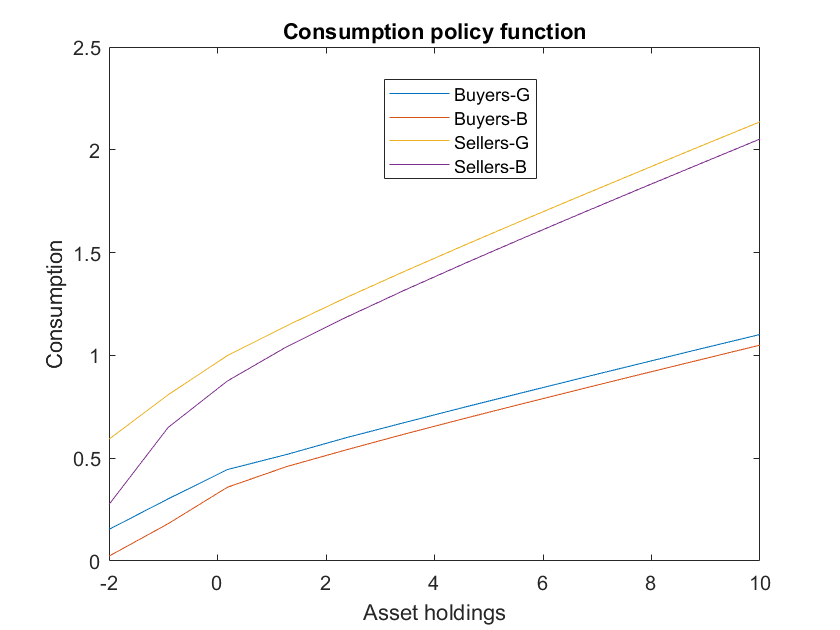
\includegraphics[angle=0,width=.5\textwidth]{figures/FIG12.png}\\ 
\multicolumn{2}{c}{(c) No Capital Income} \\  
%\multicolumn{2}{c}{(d) Equilibrium(repeated)} \\
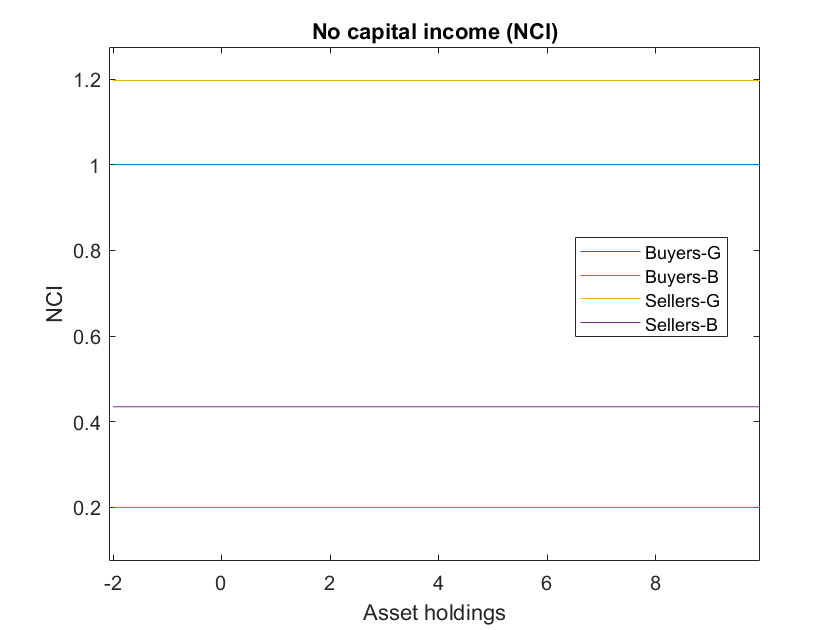
\includegraphics[angle=0,width=.5\textwidth]{figures/FIG13.png} 
%& 
%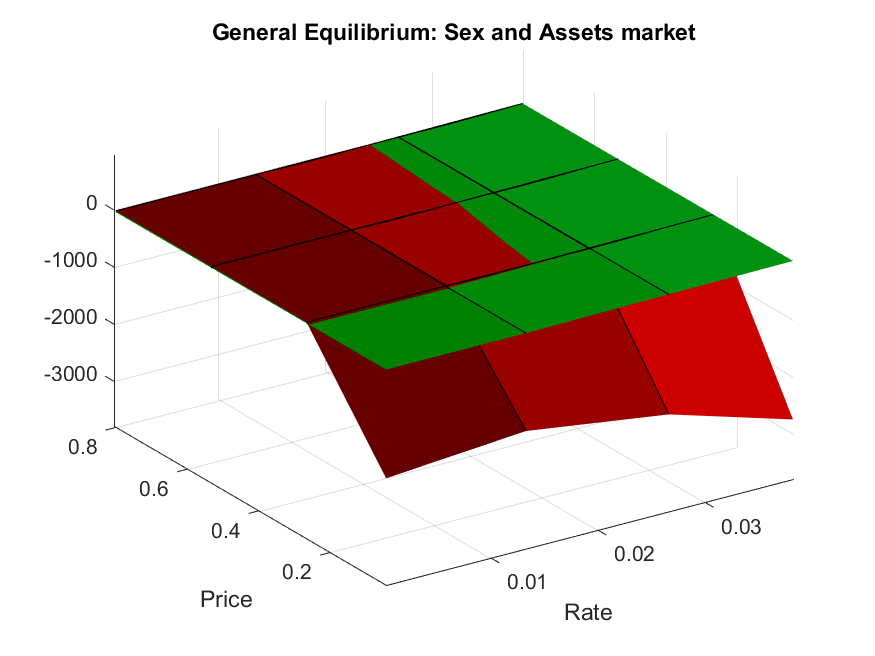
\includegraphics[angle=0,width=.5\textwidth]{figures/FIG_EQUILIBIUM3.png} 
\end{tabular}
\end{center}
\label{fig:5}
\end{figure}